\chapter*{Proposition 21}
\label{prop:21}

\begin{figure*}[ht]
    \begin{center}
    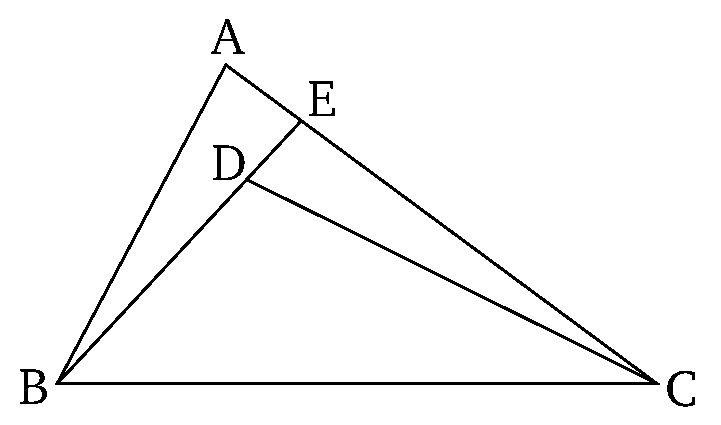
\includegraphics[width=0.5\linewidth]{figures/fig21e.eps}
    \label{fig:prop_21}
    \end{center}
\end{figure*}

If two internal straight-lines are constructed on one of the sides
of a triangle, from its ends, 
the constructed (straight-lines) will be less than the two remaining 
sides of the triangle, but will encompass a greater angle.

For let the two internal straight-lines $BD$ and $DC$ have been constructed on one of the sides $BC$ of the triangle $ABC$, from its ends $B$ and $C$ (respectively). I say that 
$BD$ and $DC$ are less than the (sum of the) two  remaining sides of the triangle
$BA$ and $AC$, but encompass an angle $BDC$ greater than $BAC$.

For let $BD$ have been drawn through to $E$. And since in any
triangle (the sum of any) two sides is greater than the remaining (side) [Prop.~1.20],
 in triangle $ABE$ the  (sum of the) two sides $AB$ and $AE$ is thus  greater than
$BE$. Let $EC$ have been added to both. Thus, (the sum of) $BA$ and $AC$ is greater
than (the sum of) $BE$ and $EC$.  Again, since in triangle $CED$ the (sum of the) two sides $CE$ and $ED$
is  greater than $CD$, let $DB$ have been added to both. Thus, 
(the sum of) $CE$ and $EB$ is greater than  (the sum of) $CD$ and $DB$. But, (the sum of) $BA$ and $AC$ was shown
(to be) greater than (the sum of) $BE$
 and $EC$. Thus, (the sum of) $BA$ and $AC$ is much greater than
(the sum of) $BD$ and $DC$.

Again, since in any  triangle the external angle 
is greater than the internal and opposite (angles) [Prop. 1.16],
 in triangle $CDE$ the external angle $BDC$ is thus greater
than $CED$.  Accordingly, for the same (reason),  the external angle $CEB$ of the
triangle $ABE$ is also greater than $BAC$. But, $BDC$ was shown (to be) 
greater
than $CEB$. Thus, $BDC$ is much greater than $BAC$.

Thus, if two internal straight-lines are constructed on one of the sides
of a triangle, from its ends, 
the constructed (straight-lines) are less than the two remaining 
sides of the triangle, but  encompass a greater angle. (Which is) the
very thing it was required to show.


\section*{Commentary}

\begin{proposition}\label{proposition_21}\lean{Elements.Book1.proposition_21}\leanok
    $D$ is a point inside $\triangle~ABC$. We have $|BD| + |DC|~<~|BA| + |AC|$, and $\angle~BDC~>~\angle~BAC$
\end{proposition}
\begin{proof}
    \uses{proposition_16,proposition_20}\leanok
    See the original proof by Euclid.
\end{proof}
